% This is now Chapter 2

\subsection{Student Feedback-Based Evaluation}
Student feedback has long been the predominant method for evaluating teaching effectiveness in higher education. Its widespread use is attributed to its simplicity, cost-effectiveness, and ability to capture students' perspectives on instructional quality \cite{Ajmal2024, Husain2016}. However, research has consistently highlighted significant limitations, including subjectivity, bias, and the influence of non-academic factors such as instructor popularity, grading leniency, and course difficulty \cite{Heffernan2022, carvalho2022biases}. Demographic factors, such as gender and race, can also affect student evaluations, raising concerns about fairness and validity \cite{Steinberg2021}. These issues have prompted calls for more objective and reliable assessment methods \cite{Ginsburg2022NecessaryBI}.

Despite its limitations, student feedback remains a central component in most institutional evaluation frameworks. Many universities rely on end-of-term surveys or online platforms to collect student opinions, which are then used for faculty appraisal, promotion, and professional development \cite{8615171}. However, the overreliance on student feedback can sometimes lead to unintended consequences, such as grade inflation or a focus on entertainment over educational rigor. Furthermore, the lack of standardization in survey instruments and interpretation of results can introduce inconsistencies across departments and institutions. Recent studies have also explored the psychological impact of student evaluations on teachers, noting increased stress and potential discouragement among faculty who receive negative or biased feedback. These findings underscore the need for complementary evaluation methods that can provide a more balanced and holistic view of teaching effectiveness.

\subsection{Auditory-Based Evaluation}
Auditory-based evaluation methods analyze audio data from classroom interactions to assess teaching performance. Techniques in this domain include speech recognition, prosody analysis, and emotion detection from vocal cues. These approaches can provide insights into teacher-student engagement, clarity of instruction, and the emotional climate of the classroom. Machine learning and signal processing advancements have enabled more accurate and automated auditory assessments, though challenges remain in handling noisy environments and diverse speaking styles \cite{Wang2022, Yang2022}.

In the context of teacher evaluation, auditory analysis offers a unique perspective by focusing on the nuances of verbal communication. For example, the tone, pace, and modulation of a teacher's voice can influence student engagement and comprehension. Studies have shown that enthusiastic and expressive speech is often associated with higher student motivation and participation. Additionally, auditory features can be used to detect classroom dynamics, such as the frequency of teacher-student interactions or the presence of collaborative discussions. Integrating auditory data with other modalities can help address the limitations of purely subjective feedback, offering a more objective measure of classroom engagement and instructional quality.

\begin{figure}[t]
    \centering
    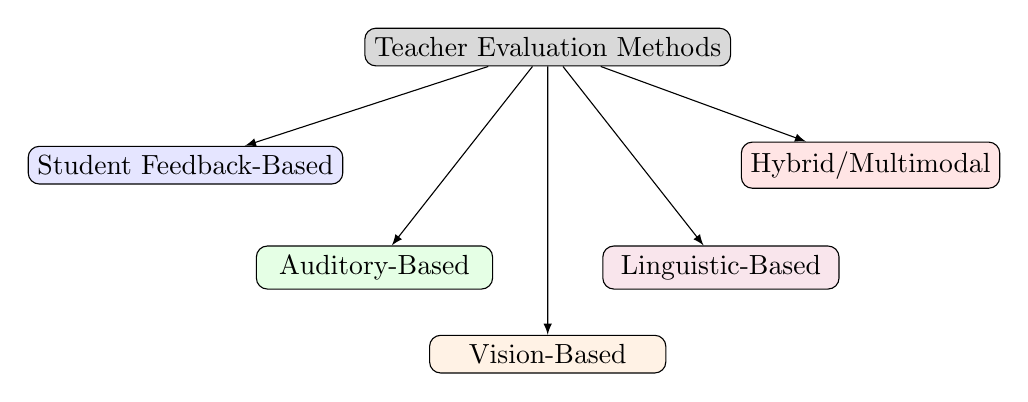
\begin{tikzpicture}[
        scale=2, % Adjusted scale for compactness
        level distance=0.8cm,
        sibling distance=1cm, % Further reduced for compactness
        every node/.style={font=\normalsize, align=center, draw, rectangle, rounded corners, minimum width=3cm, fill=gray!10},
        edge from parent/.style={draw, -latex}
    ]
    % Root node
    \node[fill=gray!30] {Teacher Evaluation Methods}
        child { node[fill=blue!10, yshift=0.1cm,xshift=-0.6cm] {Student Feedback-Based} }
        child { node[fill=green!10, yshift=-1.2cm, xshift=-0.2cm] {Auditory-Based} }
        child { node[fill=orange!10, yshift=-2.3cm, xshift=-0cm] {Vision-Based} }
        child { node[fill=purple!10, yshift=-1.2cm, xshift=0.2cm] {Linguistic-Based} }
        child { node[fill=red!10, yshift=0.1cm,xshift=0.1cm] {Hybrid/Multimodal} };
    \end{tikzpicture}
    \centering
    \caption{Taxonomy of teacher performance evaluation methods.}
    \label{fig:taxonomy}
\end{figure}


\subsection{Vision-Based Evaluation}
Vision-based evaluation leverages video data to objectively assess teacher performance. Methods include gesture recognition, pose estimation, and analysis of classroom movement patterns. These techniques capture non-verbal communication, instructional delivery, and engagement strategies. Computer vision and deep learning have significantly advanced the capabilities of vision-based systems, enabling detailed behavioral analysis in real-time classroom settings \cite{10.1007/978-981-99-9109-9_7, hou2024encouragement, Lin2021, AFSAR20156935, 10050049, YE2023108915}.

Beyond technical advancements, vision-based evaluation aligns closely with the multimodal theme of this study by providing a window into the physical and social aspects of teaching. Non-verbal cues, such as gestures, facial expressions, and movement around the classroom, play a critical role in effective pedagogy. For instance, teachers who frequently interact with students through eye contact or open body language are often perceived as more approachable and supportive. Vision-based systems can also identify patterns of classroom management, such as how teachers distribute their attention or facilitate group activities. By quantifying these behaviors, vision-based evaluation complements traditional feedback and provides actionable insights for professional development. Moreover, the integration of visual data with auditory and linguistic information can create a richer, more nuanced understanding of teaching practices.


\begin{table}[t]
    \normalsize
    \centering
    \caption{ Reliability of Teacher Evaluation Methods}
    \label{tab:reliability_methods}
    \begin{tabular}{lcc}
        \toprule
        \textbf{Method} & \textbf{Reliability} \\
        \midrule
        Student Feedback-Based & Low--Medium \\
        Auditory-Based & Medium \\
        Vision-Based & High \\
        Linguistic-Based & Medium \\
        Hybrid/Multimodal & High \\
        \bottomrule
    \end{tabular}
\end{table}

\subsection{Linguistic and Discourse-Based Evaluation}
Linguistic and discourse-based evaluation focuses on analyzing the content, structure, and sentiment of spoken or written language used by teachers. Natural language processing (NLP) techniques are employed to assess instructional clarity, discourse structure, sentiment, and the use of pedagogical language \cite{falcon2024discourse, YE2023108915, inbook, fanni2023natural, rajput2020natural, kastrati2021sentiment, jim2024recent, plaza2024emotion, karabacak2024text}. Automated discourse analysis and sentiment detection have emerged as powerful tools for evaluating communication skills and the ability to convey complex concepts. Recent studies have explored emotion analysis, topic modeling, and engagement detection in educational contexts, highlighting the growing role of NLP in teacher evaluation.

\subsection{Hybrid and Multimodal Evaluation Approaches}
Hybrid and multimodal evaluation systems integrate data from multiple sources—such as audio, video, and linguistic features—to provide a comprehensive assessment of teacher performance. These systems aim to overcome the limitations of single-modality approaches by capturing a broader range of behavioral and communicative cues. Studies have shown that multimodal systems can enhance the reliability and validity of teacher evaluations, offering more granular and actionable feedback \cite{Ginsburg2022NecessaryBI, 10.1007/978-981-99-9109-9_7, hou2024encouragement}. However, challenges remain regarding data integration, privacy, and the need for robust validation in diverse educational contexts.



As summarized in Figure~\ref{fig:taxonomy}, existing teacher evaluation methods can be broadly categorized into five main approaches, each with distinct strengths and limitations.
